% -*- coding: utf-8 -*-
 \documentclass[final,utf8,,hyperref={pdfpagelabels=false}]{beamer} 
  \mode<presentation> { 
  % \usetheme{I6dv}
  %\usetheme{I6pd}
  %\usetheme{I6pd2}
  \usetheme{LJK}
  }
  \usepackage[english]{babel}
  \usepackage[utf8]{inputenc}
  \usepackage{amsmath,amsthm, amssymb, latexsym}
  \usepackage{subfigure}
  \newcommand{\goodgap}{%
  \hspace{\subfigtopskip}%
  \hspace{\subfigbottomskip}}


  \usepackage{dg,general}
  \usepackage{tikz}

  \usetikzlibrary{arrows,shapes,mindmap}

%%
%% Colors
%%
\definecolor{grey40}{gray}{.9}
\definecolor{lbcolor}{rgb}{0.9,0.9,0.9}
\definecolor{cgreen}{rgb}{0.,0.6,0.0}

%% listings
\usepackage{listings}
\lstset{language=c++}
%\lstset{float}
\lstset{basicstyle=\small\ttfamily}
\lstset{mathescape}
\lstset{keywordstyle=\color{red}\bfseries}
\lstset{emph={val,integrate,on,grad,gradt,gradv,dot,id,dx,dy,dz,idt,dxt,dyt,dzt,div,divt,idv,dxv,dyv,dzv,dn,dnt,mass,stiffness,trans,trace,jump,jumpt,average,averaget,maxface,project,P,Px,Py,Pz,h,H,Hface,hFace,N,Nx,Ny,Nz,sqrt,sin,cos,min,max,abs,sign,pow,chi,exp,log,LinearForm,BilinearForm,MixedLinearForm,MixedBilinearForm,FESpace,MixedFESpace,
prod,element_prod, range, subrange, inner_prod,unite},emphstyle=\color{blue}}
%\lstset{stringstyle=\ttfamily}
%\lstset{commentstyle=\ttfamily\color{cgreen}}
\lstset{commentstyle=\ttfamily\color{red!25!black}}
%\lstset{numbers=left}
%\lstset{numbers={none}}
\lstset{numberstyle=\tiny}

\newcommand{\inputsnapshot}[1]{
  \lstinputlisting[frame={top,bottom}, basicstyle=\small\ttfamily]{#1}
}



  %\usepackage{times}\usefonttheme{professionalfonts}  % times is obsolete
  \usefonttheme[onlymath]{serif}
  \boldmath
  \usepackage[orientation=portrait,size=a0,scale=1.4,debug]{beamerposter}                       % e.g. for DIN-A0 poster
  %\usepackage[orientation=portrait,size=a1,scale=1.4,grid,debug]{beamerposter}                  % e.g. for DIN-A1 poster, with optional grid and debug output
  %\usepackage[size=custom,width=200,height=120,scale=2,debug]{beamerposter}                     % e.g. for custom size poster
  %\usepackage[orientation=portrait,size=a0,scale=1.0,printer=rwth-glossy-uv.df]{beamerposter}   % e.g. for DIN-A0 poster with rwth-glossy-uv printer check
  % ...
  %
  \title[Life]{Life: A Modern C++ Library for Galerkin Methods}
  \author[V. Chabannes, G. Pena \& C. Prud'homme]{V. Chabannes, G. Pena \& C. Prud'homme}
  \institute[U. Coimbra \& U. Grenoble]{U. Coimbra and U. de Grenoble}
  \date{Dec 15, 2009}
  \begin{document}
  %\usebackgroundtemplate{
\includegraphics[width=\paperwidth]{fond_ljk_diapo_seul}}
  \begin{frame}[containsverbatim]{} 
    \vfill
    %% 
    %% Start two columns
    %% 
    \begin{columns}[t]
      \column{.5\linewidth}

    \begin{block}{Introduction: Complexity in scientific computing codes}
      % \tikzstyle{root concept}+=[concept color=white!80]
      % \tikzstyle{level 1 concept}+=[concept color=ljk!80, sibling angle=90]
      % % \tikzstyle{every annotation}=[fill=black!50,opacity=0.5,text=white]
      % \begin{tikzpicture}[mindmap,concept color=black!60,text=white]
      %   \node[concept] {Complexity}
      %   [clockwise from=45]
      %   child[concept] { node[concept] (mod) {Models} }
      %   child[concept] { node[concept] (alg) {Algebraic} }
      %   child[concept] { node[concept] (cs) {Computer Science} }
      %   child[concept] { node[concept] (num) {Numerical} };
        
    % \node [annotation,left] at (mod.west)
    % {
    %   \begin{itemize}
    %   \item Geophysics
    %   \item Astrophysics
    %   \item Weather forecast
    %   \item Global Change
    %   \item Plasma physics
    %   \item Aerodynamics
    %   \item Hydrodynamics
    %   \item MHD
    %   \item Rheology
    %   \item Materials processing
    %   \item Molten metals
    %   \item Finance
    %   \end{itemize}
    % };
    % \node [annotation,left] at (sim.south west)
    % {
    %   \begin{itemize}
    %   \item Applied Mathematics
    %   \item Numerical Analysis
    %   \item Computer Science
    %   \end{itemize}
    % };
    % \node [annotation,right] at (exp.south)
    % {
    %   \begin{itemize}
    %   \item Construction d'expériences (laboratoire + numerique)
    %   \item Comparaison entre expériences en laboratoire et numériques
    %   \item Création et correction de modèles
    %   \end{itemize}
    % };

    % \begin{pgfonlayer}{background}
    %   \draw [concept connection]
    %   (exp) edge node[below,sloped,scale=.7]{Analyser,Modéliser} (mod)
    %   (mod) edge node[above,sloped,scale=.7]{Analyser,Discrétiser,Simuler} (sim)
    %   (sim) edge node[above,sloped,scale=.7]{Valider} (exp);
    % \end{pgfonlayer}

    %\end{tikzpicture}

      \begin{itemize}
      \item Algebraic (large scale nonlinear systems)
      \item Numerical (complex methods, complex meshes, etc)
      \item Models (physical laws, closure laws, etc)
      \item Computer science (parallelism, efficiency, hybrid arch, ...)
      \end{itemize}
      
      Complexity Treatments:
      \begin{itemize}
      \item Numerical and model complexity are better treated by a
        \alert{high level language}
      \item Algebraic and computer science complexity perform often better with
        \alert{low level languages}
      \end{itemize}
    \end{block}
    
    \vfill

    \begin{block}{Introduction: Generative Programming}
      \begin{itemize}
      \item Generative paradigm
        \begin{itemize}
        \item The generative paradigm is available in C++ since 1989
        \item It allows to  \alert{distribute/partition complexity}
        \item The computer science and algebraic complexity is managed by the \alert{developer}
        \item The numerical and model complexity is managed by the
          \alert{user(s)}
        \end{itemize}
      \item Definitions
        \begin{itemize}
        \item A \alert{\emph{Domain Specific Language} (DSL)} is a programming or specification language
          dedicated to a particular domain, problem and/or a solution technique
        \item A \alert{\emph{Domain Specific Embedded Language} (DSEL)}
          is a DSL integrated into another programming language (e.g. C++)
        \end{itemize}
      \end{itemize}
    \end{block}
    \vfill
%     \begin{block}{Life: Example of a DSEL -- Navier-Stokes}
%     \begin{itemize}
%     \item Life: C++ library C++ for partial differential solves developed at U. Grenoble(LJK)
%     \item We consider a Navier-Stokes solver
%       \cite{christophe09:_const_of_high_order_fluid}
%     \item The non-stabilized version reads in  C++
%       \inputsnapshot{ns.cpp}
%     \end{itemize}
%   \end{block}
%   \vfill
% \begin{block}{Life: Example of DSEL -- Stabilization}
%   \begin{itemize}
%     \item At large Reynolds number, we can, for stabilization the
%       following term \cite{Burman.Fernandez:2007},
%       \begin{equation*}
%         j_{\beta}(u, v)\eqbydef\sum_{F\in{\cal F}_h^i}\int_F
%         \left(\gamma_{\beta}+\module{\beta\SCAL n}\right)
%         \frac{h_F^2}{N^{3.5}}\jump{\GRAD u}\SSCAL\jump{\GRAD v}
%       \end{equation*}
%     \item To add it, just write
%       \inputsnapshot{stab.cpp}
%     \end{itemize}
%   \end{block}

    \begin{block}{Some Mathematical Features}
      \begin{itemize}
      \item Support 1D, 2D, 3D and basic entities: simplices and product of simplices
      \item Support various point sets on these basic entities: equidistributed
        points, quadrature points, interpolation points (Gauss-Lobatto, Fekete,
        WarpBlend, Electrostatic)
      \item Support various polynomial sets (Lagrange, Dubiner/BA, Legendre/BA,
        \dots)
        % \begin{itemize}
        % \item Lagrange(continuous,discontinuous,all dimensions,all interpolation point sets)
        % \item Dubiner(discontinuous), boundary adapted(continuous)
        % \item Legendre(discontinuous), boundary adapted(continuous)
        % \end{itemize}
      \item Support continuous and discontinuous Galerkin methods
      \item Support for parallel computation and interfaces to GMM, PETSc/SLEPc,
        Trilinos
        % \item Provide mathematical concept for higher order abstraction
      \item Interpolation in 1D, 2D, 3D
      \item Provide a domain specific language embedded in C++ ala FreeFem++
        thanks to generative programming.
      \end{itemize}
    \end{block}

    \begin{block}{Ingredients}
      \centerline{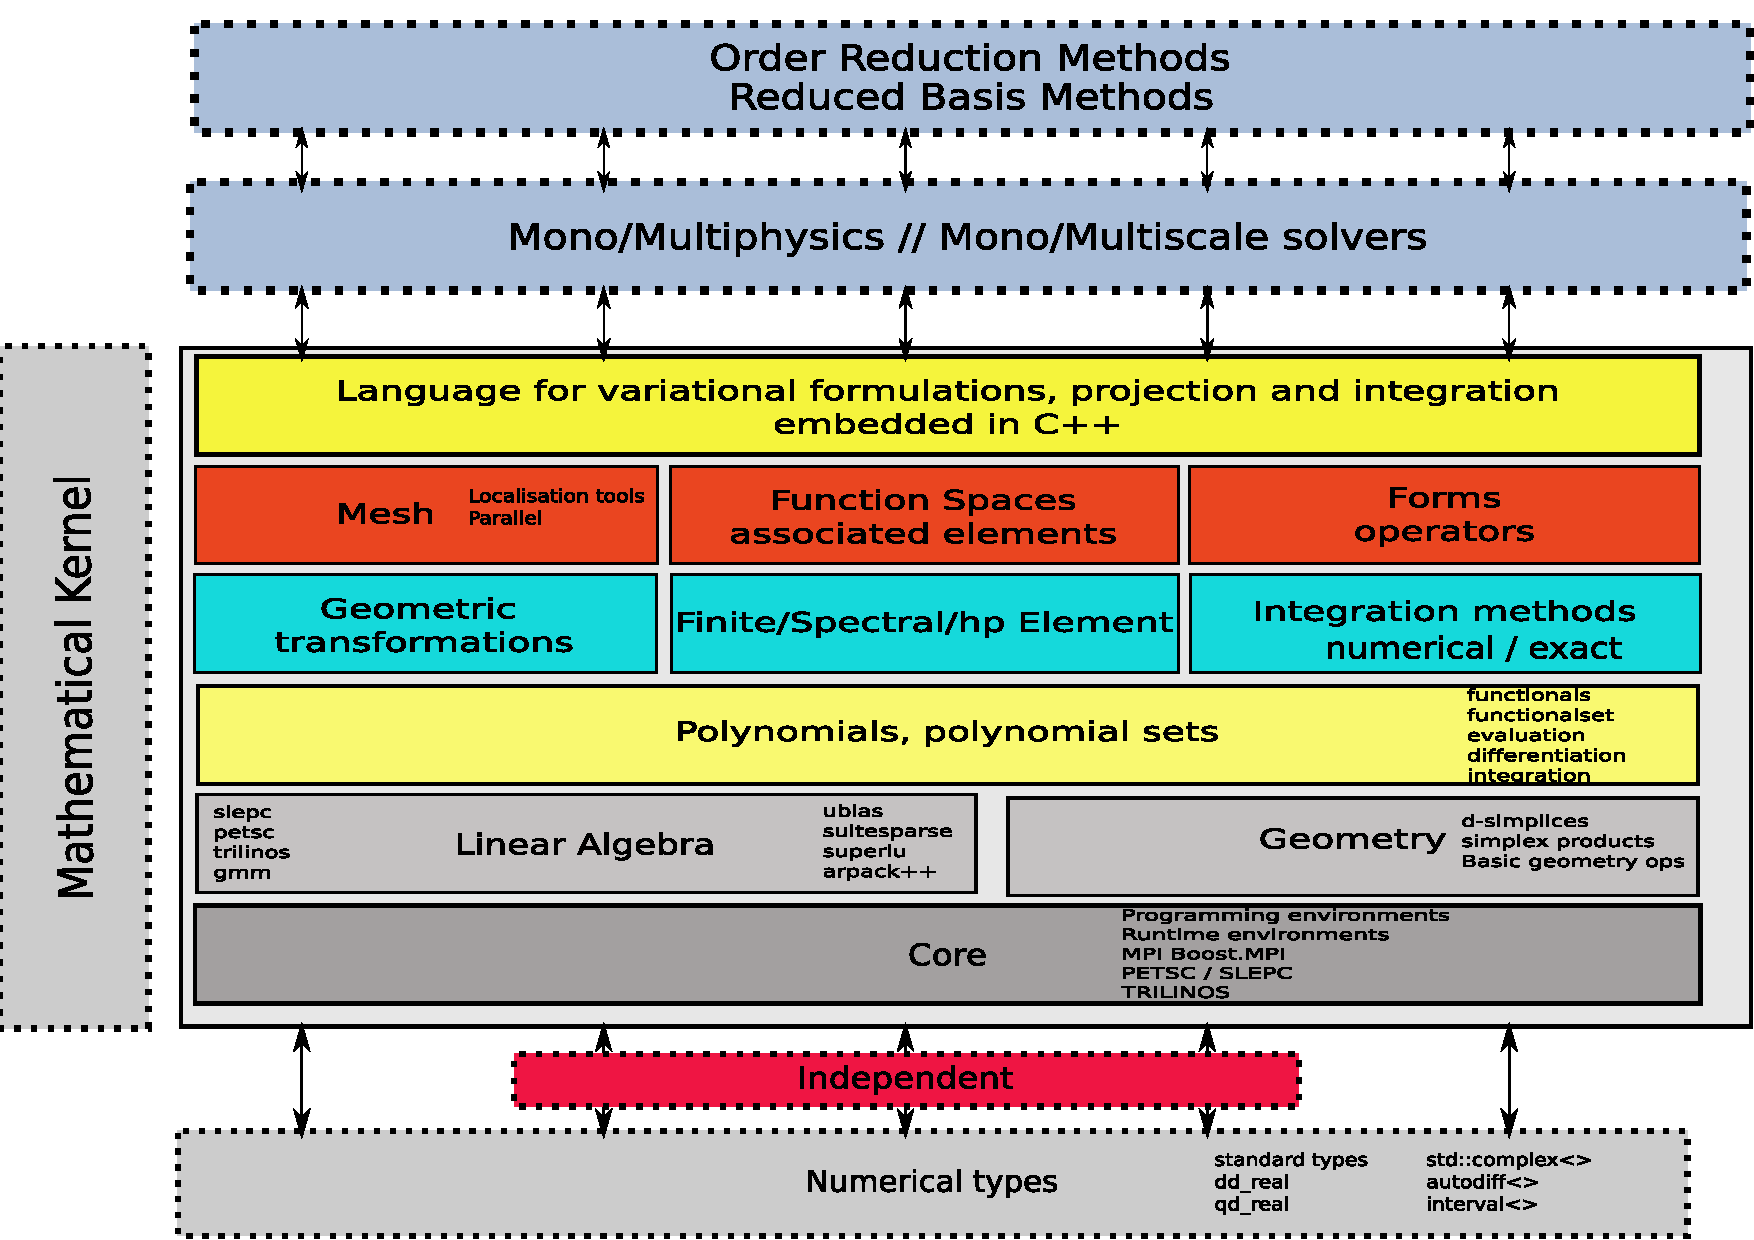
\includegraphics[width=\linewidth]{arch2.pdf}}
    \end{block}
    \vfill
    \begin{block}{Life: A Language for PDEs -- Navier-Stokes and Heat Transfer}
   
      
      \tikzstyle{mybox} = [draw=gray!10!white!, fill=gray!10!white, very thick,
      rectangle, rounded corners, inner sep=10pt, inner ysep=20pt]
      \tikzstyle{fancytitle} =[draw=gray,fill=gray!10!white, text=red, ellipse]
      % 
      \begin{tikzpicture}[transform shape, baseline=-3.5cm]
        \node [mybox] (box) {%
        \begin{minipage}{.94\textwidth}
         \begin{columns}[t]
        \begin{column}{.55\textwidth}  
          \begin{lstlisting}
 //standard terms for NS
 integrate( elements(mesh), 
    $\nu$*trace(gradt(u)*trans(grad(v)))
  + trans(idt(u))*id(v)/dt
  + ($\beta$*trans(gradt(u)))*id(v) 
  - idt(p)*div(v) + id(q)*divt(u))
 // stab. for equal-order approx.
 + integrate(internalfaces(mesh), 
   maxface($\gamma$*pow(h(),3)/max(h()*
     sqrt(trans($\bf\beta$)*($\bf\beta$)), $\nu$))
   * ( jump(grad(q)*N())*jumpt (gradt(p)*N())));
\end{lstlisting}
\end{column}
\begin{column}{.52\textwidth}
\begin{figure}[H]
\centering
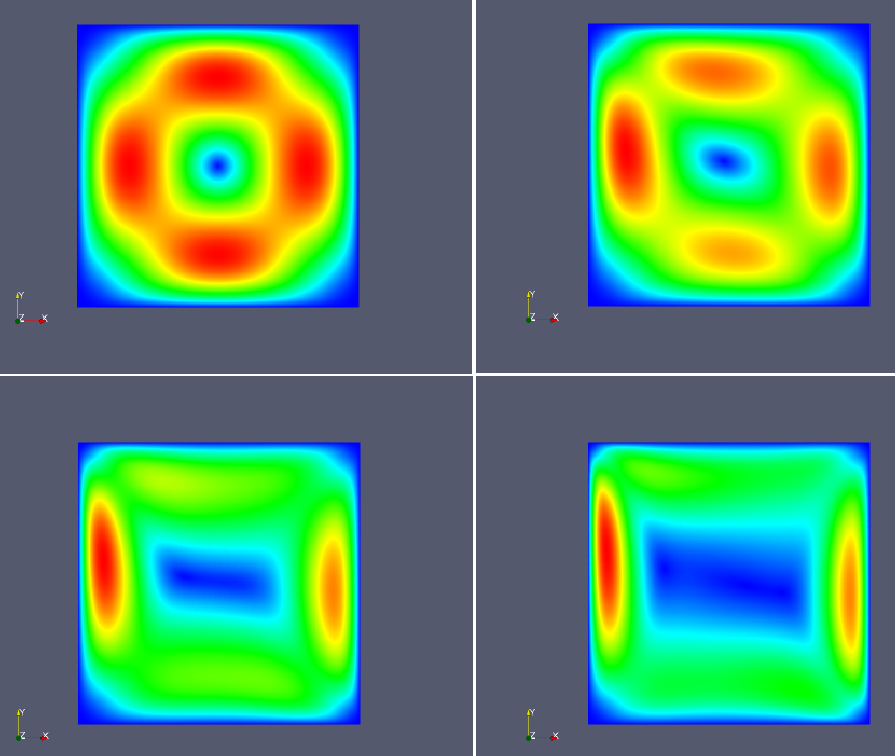
\includegraphics[width=.6\linewidth,height=0.4\linewidth]{../tutorial/pngs/flow_grashof}
\caption{Natural convection: flow field for different values of the Grashof number.}
\end{figure}
    \end{column}
      \end{columns}
      \end{minipage}
      };
      \node[fancytitle] at (box.north) {Example: The Navier-Stokes code };
    \end{tikzpicture}
    
    
  \end{block}

%%%%%%%%%%%%%%%%%%%%%%%%%%%%%%%%%%%%%%%%%%%%%%%%%%%%%%%%%%%%%%%%%%%%%%%%%%%%%%%%%%
%% 2nd column of the Poster
%%%%%%%%%%%%%%%%%%%%%%%%%%%%%%%%%%%%%%%%%%%%%%%%%%%%%%%%%%%%%%%%%%%%%%%%%%%%%%%%%%
    \column{.5\linewidth}
    \vfill

  \begin{block}{Life: A Language for PDEs -- Linear Elasticity}
      \tikzstyle{mybox} = [draw=gray!10!white!, fill=gray!10!white, very thick,
  rectangle, rounded corners, inner sep=10pt, inner ysep=20pt]
  \tikzstyle{fancytitle} =[draw=gray,fill=gray!10!white, text=red, ellipse]
  %
  \begin{tikzpicture}[transform shape, baseline=-3.5cm]
    \node [mybox] (box) {%
      \begin{minipage}{.94\textwidth}
\lstset{escapechar=@}
%//Identity matrix
%auto( Id , oneX()*trans(oneX()) + oneY()*trans(oneY()) ); @\vspace{0.3cm}@
%//Gradient des deformations $F = Id + \nabla u$
%//Tenseur de Green-Lagrange : $E=\frac{1}{2}\left( \nabla u + \left(\nabla u\right)^{T} \right) + \frac{1}{2}\left( \left(\nabla u\right)^{T} \nabla u \right)$
%//Loi de comportement St-Venant-Kirchhoff : $S = \lambda tr\left(E\right) Id + 2 \mu E$
%//Force volumique
%//$-\int_{\Omega} FS:\nabla v + \int_{\Omega} \rho \ \eta \vec{n_{y}} \cdot v$ + C.L.
\vspace{0.3cm}
\begin{lstlisting}
auto F=Id + gradv(u); auto S=lambda*trace(E)*Id + 2*mu*E;
auto E=0.5*(gradv(u)+trans(gradv(u))+trans(gradv(u))*gradv(u)); 
auto $\eta$=(Px()-0.4)*(Px()-0.45)*chi(Px()>=0.4 && Px()<=0.45); @\vspace{0.3cm}@
form1( Xh, R ) = integrate( elements(mesh),
 - trace((F*S)*trans(grad(v))) + trans($\rho \eta \vec{\jmath}$)*id(v) )
 + on( markedfaces(mesh,"clamped"), u, R, constant(0)*one() ); @\vspace{0.3cm}@
\end{lstlisting}
%// move the mesh according the displacement $u$
%MeshMover<mesh_type> meshmove;
%meshmove.apply( mesh, u );

      \end{minipage}
      };
      \node[fancytitle] at (box.north) {Example: a Nonlinear-Elasticity code : Residual Part};

    \end{tikzpicture}
\begin{figure}[H]
\centering
\label{fig:schemaint}	

\includegraphics[width=.9\linewidth]{structure}
\caption{A clamped Saint-Venant Kirchhoff structure.}
\end{figure}


  \end{block}


  \begin{block}{Applications: Navier-Stokes incompressible Multi-Fluid}
    
    \begin{columns}[t]
      \begin{column}{.45\textwidth}
        \begin{figure}
      \centering
      \subfigure[$t=2$]{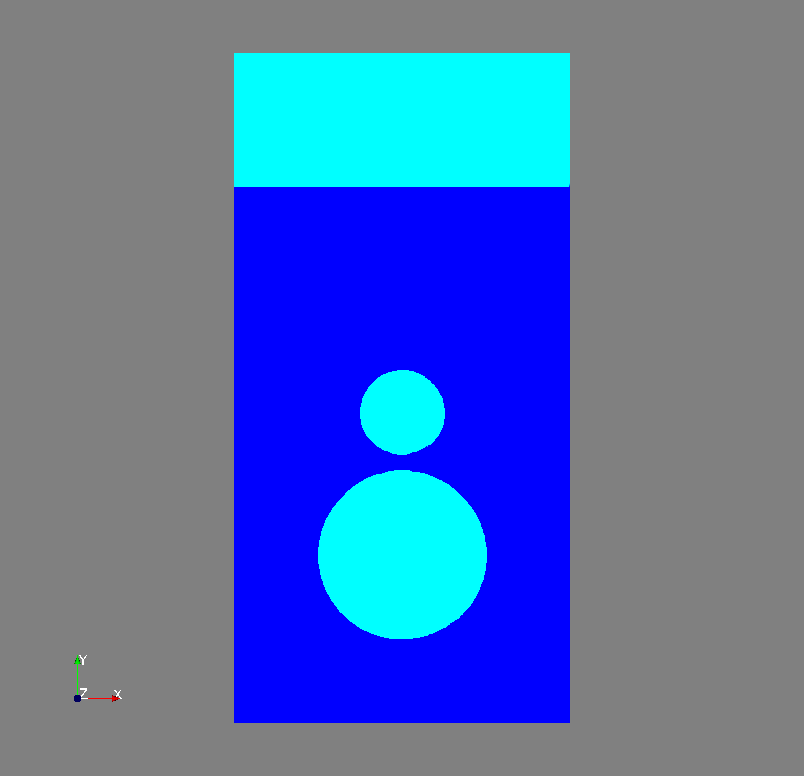
\includegraphics[width=.4\linewidth]{duebolle2-2}}\goodgap
      \subfigure[$t=20$]{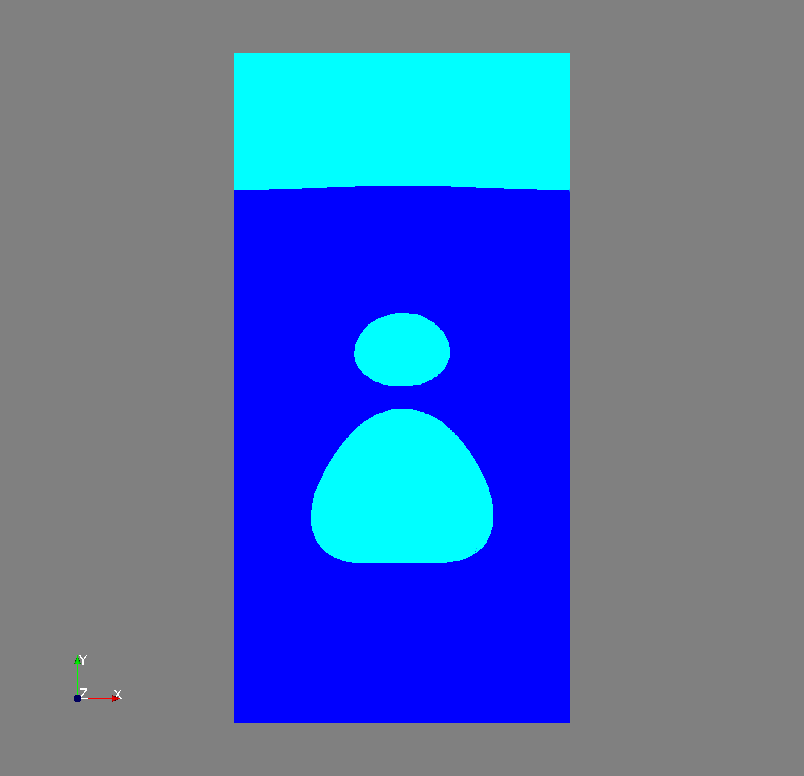
\includegraphics[width=.4\linewidth]{duebolle2-20}}\\
      \subfigure[$t=30$]{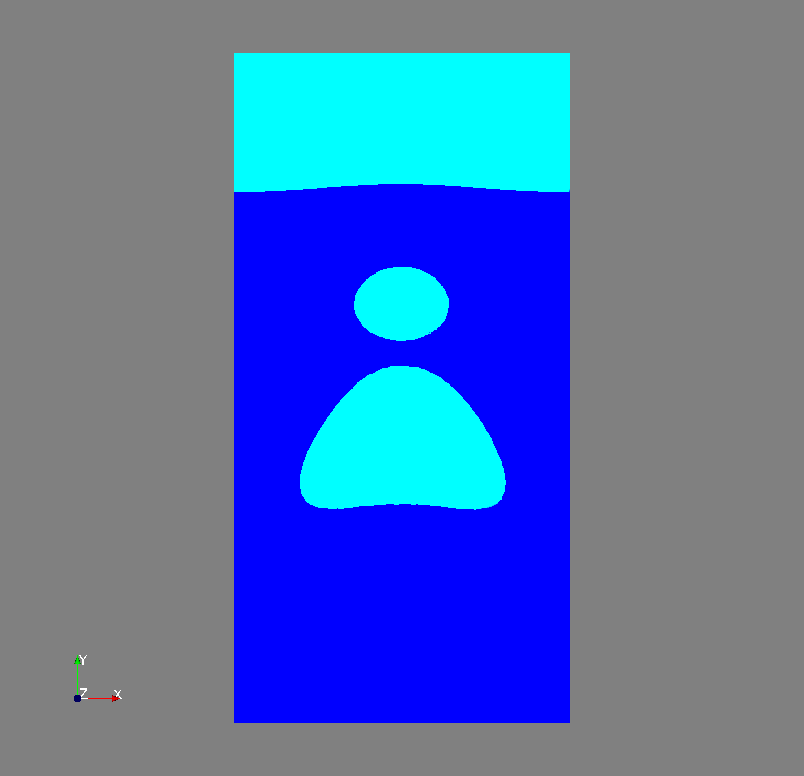
\includegraphics[width=.4\linewidth]{duebolle2-30}}\goodgap
      \subfigure[$t=50$]{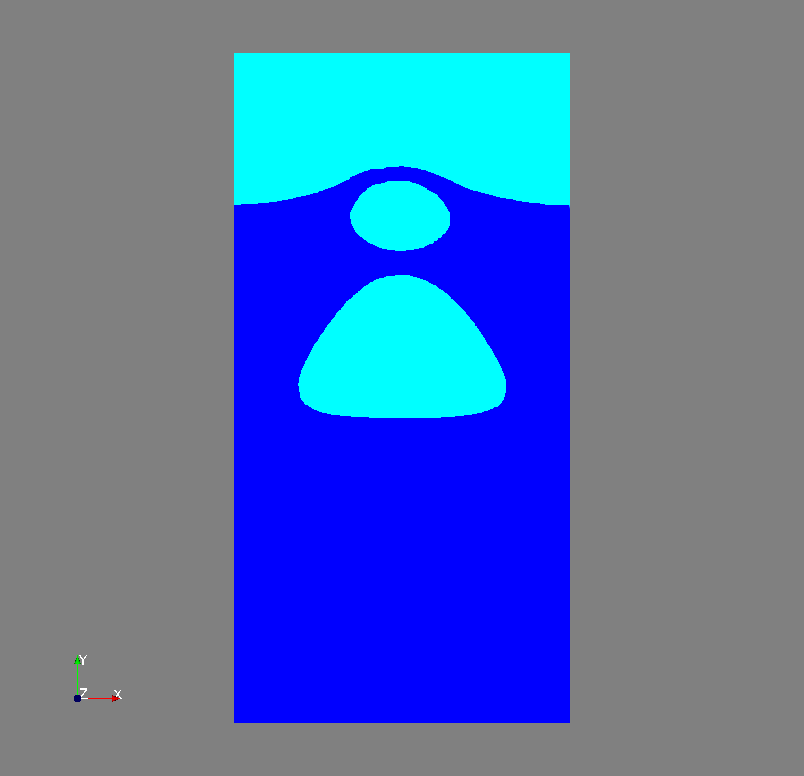
\includegraphics[width=.4\linewidth]{duebolle2-50}}\\
      \subfigure[$t=70$]{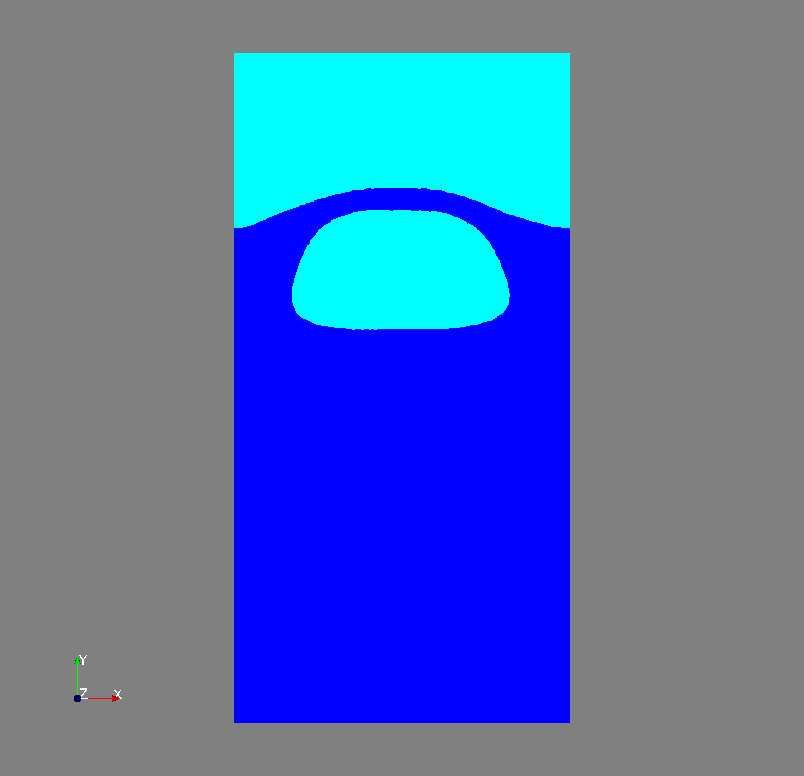
\includegraphics[width=.4\linewidth]{duebolle2-70}}\goodgap
      \subfigure[$t=90$]{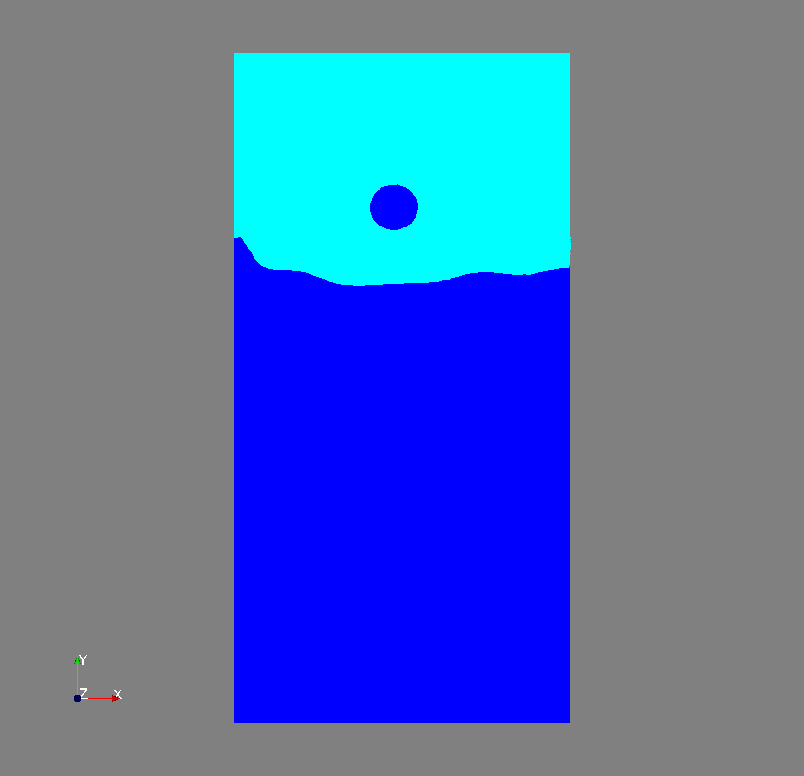
\includegraphics[width=.4\linewidth]{duebolle2-90}}
      \caption{Two bubbles (coutersy of C. Winkelmann).}
      \label{fig:1}
    \end{figure}
      \end{column}
      \begin{column}{.52\textwidth} \vspace*{-1cm}
          \begin{block}{Navier-Stokes Bi-Fluid}
            \begin{itemize}
            \item N(=2) incompressible fluid flows
            \item Navier-Stokes equations in all  $\Omega$
            \item Variable density and viscosity
              
            \item Advection of the level set function
            \item Explicit determination of the interface
            \item Integration on the interface (surfacic tension)
            \item Reinitialisation of the  level set function
              
            \item Fixed point iterations for all nonlinearities
            %\item P2/P1 not stabilized for NS and P1 stabilized for CIP for levelset
              
            \item Changes in topology: 2 bubles (a-d) 1 buble (e), 1 droplet (f)
            \item Filament in (e) takes back the form of a circular bubble due
              to surfacic tension

            \item Quantities of the benchmark recovered reliably
            \item Skirt formation
            \end{itemize}
          \end{block}
        \end{column}
      \end{columns}

  \end{block}

  \begin{block}{Applications: Fluid-Structure Interaction in Hemodynamics}
    
    \begin{columns}[c]
      \begin{column}{.40\linewidth}
        %\vspace{-1cm}
        \begin{figure}
          \begin{minipage}[b]{0.6\linewidth} % A minipage that covers half the page
            \centering
            \subfigure[$t=0ms$]{
\includegraphics[width=.8\linewidth]{figures/pressure_wave_magnify_0000}} \vspace{0.5cm}\\
            \subfigure[$t=2ms$]{
\includegraphics[width=.8\linewidth]{figures/pressure_wave_magnify_0004}} \vspace{0.5cm}\\
            \subfigure[$t=4ms$]{
\includegraphics[width=.8\linewidth]{figures/pressure_wave_magnify_0008}} \vspace{0.5cm}\\
            \subfigure[$t=6ms$]{
\includegraphics[width=.8\linewidth]{figures/pressure_wave_magnify_0012}} \vspace{0.5cm}\\
            \subfigure[$t=8ms$]{
\includegraphics[width=.8\linewidth]{figures/pressure_wave_magnify_0016}} \vspace{0.5cm}\\
            \subfigure[$t=10ms$]{
\includegraphics[width=.8\linewidth]{figures/pressure_wave_magnify_0020}}
          \end{minipage}
          \begin{minipage}[t]{0.25\linewidth}
            \centering
            \subfigure[Legend]{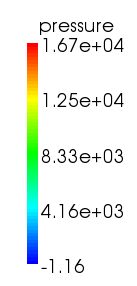
\includegraphics[width=4cm]{figures/pressure_wave_magnify_legend}}
          \end{minipage}
          \caption{Pressure pulse travelling through the artery}
          \label{pressure_wave}
        \end{figure}
        
        
      \end{column}
      \begin{column}{.55\textwidth}
        \vspace{-2.5cm}
        \begin{block}{Navier-Stokes + generalized string}
          \begin{itemize}
	      \item Fix point method for fully coupled problem
	      \item Semi-implicit method approach
	      \item Triangular spectral elements in space
% 	      \item Continuous Galerkin setting
	      \item High order schemes in time: BDF, AFM
	      \item High order mesh couples structure and fluid
	      \item Aitken relaxation strategy
          \end{itemize}
        \end{block}
        \begin{block}{Properties (fix point iterations)}
          \begin{itemize}
	      \item unchanged wrt $k$, using $\mathbb P_k$ - $\mathbb P_{k-2}$
	      \item increases, with increased $N_{geo}$
	      \item decreases, increasing  BDF order for the structure
	      \item increases, increasing BDF order for the fluid
          \end{itemize}
        \end{block}
      \end{column}
    \end{columns}
  \end{block}
  \vfill

      \begin{block}{More information}
      \begin{itemize}
      \item Contributors:
        \begin{itemize}
        \item LJK/EDP, Université Joseph Fourier Grenoble 1
        \item CMCS, EPF Lausanne (Switzerland)
        \item CMUC, U. Coimbra (Portugal)
        \end{itemize}
      \item Usage Contexts:
        \begin{itemize}
        \item Research: Numerical rheology of blood in arteries, certified
          reduced basis...
        \item Teaching and projects at Master level
        \item Industrial contracts: ANR OPUS(EADS), IFP
        \end{itemize}
      \end{itemize}
    \end{block}

  \end{columns}
  \end{frame}





  \end{document}
